\section{Kompressionsstandard Brotli-G}
\label{sec:brotlig}
In vielen Anwendungsfällen wird auf Kombinationen von Kompressionsalgorithmen gesetzt.
[QUELLE für Kompression]
Auch Brotli macht sich mehrere Algorithmen zunutze.
Google hat für die Entwicklung von Brotli eine eigene Implementierung des Deflate Algorithmus verwendet.
Das Ergebnis der Kompression besteht aus einer Reihe an Meta Blöcken.
Anstelle der kompletten Daten teilt Brotli den Datensatz in logische Blöcke ein, damit ein besseres Kompressionsergebnis erzielt werden kann.
So wird jeder dieser Blöcke einzeln komprimiert, und zusammen mit den Header Informationen für die gesamten Daten in das Brotli Format geschrieben.
Um die Daten zu komprimieren wird eine Kombination des LZ77 Algorithmus verwendet, um duplizierte Zeichenketten zu erkennen, und einer Huffman-Kodierung um Präfix freie Codewörter zu generieren.
Jeder Meta Block hat dabei seine eigene Huffman-Kodierung.
So sind Überschneidungen von Codewörtern in unterschiedlichen Meta Blöcken möglich, während ein Präfix freier Code in einem Meta Block gewährleistet ist.
Der LZ77 Algorithmus hat zusätzlich noch die Möglichkeit, in einem zuvor kodierten Meta Block nach duplizierten Zeichenketten suchen, sollte diese Zeichenkette noch im Schiebefenster vorhanden sein \cite{rfc7932}. \newline

Um eine parallele Dekompression zu ermöglichen, musste AMD bei Brotli-G einige Veränderungen an den Algorithmen vornehmen.
Zum einen kann die Größe des Schiebefensters abweichen.
Das kommt auf die Größe der Eingabedaten an.
Um die Parallelisierung der Dekompression zu gewährleisten muss auf die Verwendung von vorherigen Meta Blöcken verzichten, und das Schiebefenster zu Beginn eines neuen Meta Blocks zurücksetzen \cite{AMD2024}. \newline

Um die verwendeten Algorithmen besser zu verstehen werden sie in den folgenden Kapiteln genauer betrachtet.

\subsection{LZ77}
\label{subsubsec:lz77}
Der LZ77 (\textit{Lempel-Ziv77}) Algorithmus gehört zu der Gruppe der Phrasenkodierung und ist ein verlustfreier, auf einem Wörterbuch basierender Algorithmus.
Der Algorithmus komprimiert sequentielle Zeichenketten.
Dabei kann dieser auf jeder Art von Daten, egal wie der Inhalt und die Größe aussieht, angewendet werden.
Ob es sich lohnt, diesen anzuwenden, ist jedoch von den Daten abhängig.
Beispielsweise sind Bilder ein schlechter Anwendungsfall, da sich die Informationen nur im Ausnahmefall wiederholen, und es deutlich bessere Kompressionsalgorithmen zur Komprimierung dieser gibt.
Das Ziel des LZ77 Algorithmus ist lediglich, redundante Informationen zusammenzufassen. \newline

Bevor der Algorithmus beschrieben wird, werden die benötigten Elemente definiert:

\begin{enumerate}
\item{Eingabestrom:} Die zu kodierenden Daten
\item{Symbol:} Ein willkürlich gewähltes Element des Eingabestroms
\item{Datenfenster:} Alle Symbole vom Start des Eingabestroms bis zum aktuell betrachteten Symbol
\item{Vorschaufenster:} Ein Buffer fester Größe der Symbole vom aktuell betrachteten Symbol bis zum Ende des Buffers enthält
\item{Schiebefenster:} Daten- und Vorschaufenster
\item{Codewort:} Ein Codewort bestehend aus dem Offset, der Lauflänge und des zu kodierenden Symbols
\end{enumerate}

Der Ablauf des Algorithmus besteht aus folgenden Schritten:

Zu Beginn des Algorithmus wird das Datenfenster auf den Start des Eingabestroms gesetzt.
Dieses Fenster ist zunächst leer.
Das Vorschaufenster wird vom Start des Eingabestroms mit Symbolen gefüllt, bis dieses voll ist.
Zunächst wird das erste Symbol kodiert.
Dafür verwendet der LZ77 Algorithmus ein Tupel in der Form von (\textit{Position}, \textit{Lauflänge}) und abschließend das zu kodierende Symbol.
Dem Wörterbuch noch nicht bekannt Symbole werden neue Symbole mit (0, 0)Symbol hinzugefügt.
Nach jedem Schritt wird das Schiebefenster um die Lauflänge der kodierten Symbole im Eingabestrom verschoben
\cite{lz2023}.

\subsubsection{Kodierung eines Codewortes}
\label{subsubsec:kodierung_codewort}
Zur Veranschaulichung wird das Codewort \glqq laufenraufen\grqq\ mit dem LZ77 Algorithmus kodiert und anschließend wieder dekodiert.
Daten- und Vorschaufenster haben in diesem Beispiel eine Kapazität von jeweils sechs Symbolen. \newpage
\begin{table}[H]
\centering
\begin{tabular}{|l|l|l|l|}
\hline
\textbf{Datenfenster} & \textbf{Vorschaufenster} & \textbf{restliches Codewort} & \textbf{Kodierung} \\ \hline
                      & laufen                   & raufen                       & (0, 0)l            \\ \hline
l                     & aufenr                   & aufen                        & (0, 0)a            \\ \hline
la                    & ufenra                   & ufen                         & (0, 0)u            \\ \hline
lau                   & fenrau                   & fen                          & (0, 0)f            \\ \hline
lauf                  & enrauf                   & en                           & (0, 0)e            \\ \hline
laufe                 & nraufe                   & n                            & (0, 0)n            \\ \hline
laufen                & raufen                   &                              & (0, 0)r            \\ \hline
aufenr                & aufen                    &                              & (6, 4)n            \\ \hline
\end{tabular}
\label{tab:lz77_encode_table}
\caption{LZ77 Kodierungs Beispiel}
\end{table}

Eine Besonderheit die zunächst nicht intuitiv ist, ist die Konstruktion des letzten Codewortes in diesem Beispiel.
Die Symbolsequenz \glqq aufen\grqq\ mit der Kodierung \textit{(6, 4)n} könnte auch mit einem Offset von fünf kodiert werden.
Im Normalfall würde die Symbolsequenz auch so kodiert werden.
Da jedoch das Symbol \glqq n\grqq\ das letzte Symbol des zu kodierenden Worts ist, und es so kein weiteres, zu kodierendes Symbol gibt, muss die Länge um eins reduziert werden, und das letzte Symbol kodiert werden. \newline

Aus dem Beispiel geht hervor, das die Auswahl der Buffergröße gut gewählt werden muss, damit der Algorithmus effektiv verwendet werden kann.
Wäre in dem Beispiel das Datenfenster lediglich Platz für vier statt fünf Symbole, hätte die Symbolsequenz \glqq aufe\grqq nicht als ganzes kodiert werden können.
Die weiteren Iterationen der Lempel-Ziv Algorithmen haben statt einem lokalen Wörterbuch (Datenfenster) ein globales Wörterbuch verwendet.
Durch die große Anzahl an Vergleichen erreicht der LZ77 Algorithmus ein besseres Kompressionsverhältnis als der LZ78 Algorithmus, benötigt für die Kompression jedoch länger.
Wie lange das Komprimieren der Daten dauert ist jedoch nicht wichtig für diese Arbeit.
Der interessante Punkt ist die Dekompressionsgeschwindigkeit.
Der LZ77 Algorithmus ist bedeutend schneller bei der Dekomprimierung als bei der Komprimierung \cite{Choudhary2015}. \newpage

\subsubsection{Dekodierung eines Codeworts}
\label{subsubsec:dekodierung_codewort}
In diesem Abschnitt soll aus der Kodierung das zuvor festgelegte Codewort dekodiert werden.
Als Ergebnis aus der Kodierung erhalten wir den Ausgabestrom: \newline
 \textit{(0, 0)l}, \textit{(0, 0)a}, \textit{(0, 0)u}, \textit{(0, 0)f}, \textit{(0, 0)e}, \textit{(0, 0)n}, \textit{(0, 0)r}, \textit{(6, 4)n}. \newline
Jetzt gilt es, das Datenfenster zu füllen.
In einem Schritt der Dekodierung wird das Datenfenster überprüft, sollte Offset und Lauflänge ungleich 0 sein.
Falls vorhanden werden die Daten des Datenfensters mit dem Symbol der aktuell zu dekodierenden Symbol dem Codewort hinzugefügt.
Im nächsten Schritt wird die Symbolsequenz an die Symbole des Datenfensters verkettet, bis dieses voll ist.
Anhand des letzten Schrittes der Dekompression sieht man wie der Algorithmus eine duplizierte Zeichenkette erkennt.
In diesem Beispiel wird die Zeichenkette \textit{aufe} mit einem Offset von 6 und einer Lauflänge von 4 aus dem Datenfenster gelesen, und mit dem Symbol \textit{n} verkettet.
Die Dekodierung ist nach diesem Schritt abgeschlossen.
\newline
\begin{table}[H]
\centering
\begin{tabular}{|l|l|l|}
\hline
\textbf{Kodierung} & \textbf{Datenfenster}         & \textbf{Codewort} \\ \hline
(0, 0)l            &                               & l                 \\ \hline
(0, 0)a            & l                             & la                \\ \hline
(0, 0)u            & la                            & lau               \\ \hline
(0, 0)f            & lau                           & lauf              \\ \hline
(0, 0)e            & lauf                          & laufe             \\ \hline
(0, 0)n            & laufe                         & laufen            \\ \hline
(0, 0)r            & laufen                        & laufenr           \\ \hline
{\color[HTML]{009901}(6, 4)n}            & {\color[HTML]{009901} aufe}nr & laufenr{\color[HTML]{009901} aufen}      \\ \hline
\textbackslash 0   & raufen 					   & laufenraufen 		\\ \hline
\end{tabular}
\label{tab:lz77_decode_table}
\caption{Dekodierung mit dem LZ77-Algorithmus}
\end{table}

Wie zu sehen ist, ist der LZ77 Algorithmus sowohl leicht verständlich als auch effektiv, wodurch er seinen Nutzen in vielen Anwendungen findet.
Seine Weiterentwicklungen nennen sich LZ78 und LZW, die zwar dem LZ77 Algorithmus technisch überlegen sind, aufgrund von Patenten jedoch nicht so eine große Rolle spielen wie die erste Iteration von Lempel und Ziv.
In Kombination mit anderen Techniken wie der Huffman Codierung bildet der LZ77-Algorithmus jedoch die Grundlage vieler leistungsstarker Kompressionsstandards, die heute in vielen Applikationen zu finden sind [QUELLE!!!]. \newline


\subsection{Huffman-Kodierung}
\label{subsec:huffman}
Eine gewisse Ähnlichkeit zu dem in der Einleitung angerissenen Thema des Morse Codes enthält die von Brotli verwendete Huffman-Kodierung.
Die Huffman-Kodierung ist eine Methode zur verlustfreien Datenkompression und gehört zur Art der Codewort basierten Entropiekodierung.
Ähnlich wie beim Morse Code, werden Symbole durch Bitfolgen substituiert.
Was beim Morse Code als langes und kurzes Signal galt, ist im Huffman Code eine 0 oder 1.
Mit der Huffman-Kodierung werden häufig auftretende Symbole durch kurze Bitfolgen dargestellt.
Dementsprechend erhalten Symbole mit geringer Auftrittswahrscheinlichkeit ein langes Codewort.
Bei der Betrachtung des Morse Codes fällt auf, dass nicht jeder Buchstabe die selbe Anzahl an Signalen beansprucht.
Die Codewörter im Morse Code haben sich nämlich ebenfalls die Eigenschaft der Auftrittswahrscheinlichkeiten zunutze gemacht.
Die im englischen Alphabet meist verwendeten Codewörter \glqq E\grqq\ und \glqq T\grqq\ werden beide mit jeweils einem Signal dargestellt.
Das \glqq E\grqq\ wird mit einem kurzen, während das \glqq T\grqq\ vom langen Signal dargestellt wird.
Mithilfe dieser Eigenschaft verbrauchen Symbole, die häufig auftreten, weniger Platz im Bitstrom \cite{Moffat2019}.
Histogramm ....

\subsubsection{Konstruktion einer Huffman-Kodierung}
\label{subsubsec:konstruktion_huffman}
Zur Konstruktion eines Huffman Codes wird ein Binärbaum generiert.
Die zu kodierenden Symbole werden als Blätter des Baumes betrachtet.
Der Baum wird sozusagen von \glqq unten nach oben\grqq\ bzw. von \glqq Blätter nach Wurzel\grqq aufgebaut. \newline
In jedem Schritt werden die zwei Symbole oder Knoten mit der geringsten Auftrittswahrscheinlichkeit zu einem neuen Knoten verbunden.
Die Auftrittswahrscheinlichkeit des neu erstellten Knotens ist die Summe der Auftrittswahrscheinlichkeiten der verbundene Symbole/Knoten.
Sobald die Wurzel des Baumes erreicht ist, also die Auftrittswahrscheinlichkeit bei 1 liegt, ist die Huffman-Kodierung abgeschlossen.
Jedem Zweig des Baums wird zusätzlich eine 0 oder 1 zugewiesen.
Ob der linke Kindknoten die 0 und der rechte Kindknoten die 1 bekommt, oder anders herum ist nicht wichtig, und kann von Implementierung zu Implementierung abweichen.
Wichtig ist nur zu beachten, das dies im gesamten Baum konsistent durchgezogen wird.
Die Codewörter für jedes Symbol sind abzulesen, indem die Beschriftungen der Zweige als ein Bitstrom interpretiert werden, beginnend von der Wurzel.

Um den Vorteil dieser Eigenschaft zu Veranschaulichen, kann ein Vergleich mit dem \textit{fixed length Code (FLC)} hilfreich sein.
Anders als \textit{Variable Length Code (VLC)} Verfahren wie die Huffman-Kodierung, wird jedem Symbol eines FLCs ein Codewort fester Länge zugewiesen.
Die Auftrittswahrscheinlichkeit spielt bei der Erstellung von Codewörtern also keine Rolle.
Um einen Vergleich zu ziehen kann die mittlere Codewortlänge des Alphabets, mit folgenden Symbolen betrachtet werden.

\begin{table}[h]
\centering
\begin{tabular}{ccccc}
\toprule
\textbf{\textit{\(S_i\)}} & {A} & {B} & {C} & {D} \\
\midrule
\textbf{\textit{\(P_i\)}} & 0.6 & 0.2 & 0.1 & 0.1\\
\bottomrule
\end{tabular}
\end{table}

Die Formel zur Berechnung der mittleren Codewortlänge des FLCs lautet
\begin{equation*}
\bar{l} = \lceil \log_2(N) \rceil
\end{equation*}
Wird das aus 4 Symbolen bestehende Beispielalphabet mittels FLC kodiert, ist die Codewortlänge \(l_i\) eines jeden Symbols = 2, wodurch auch die mittlere Codewortlänge bei 2,0 \textit{Bits/Symbol} liegt.

Die Konstruktion des Binärbaums, aus dem die Codewörter entnommen werden können ist in Abb.~\ref{fig:huffman_example} zu sehen.

\begin{figure}[htb]
  \centering  
  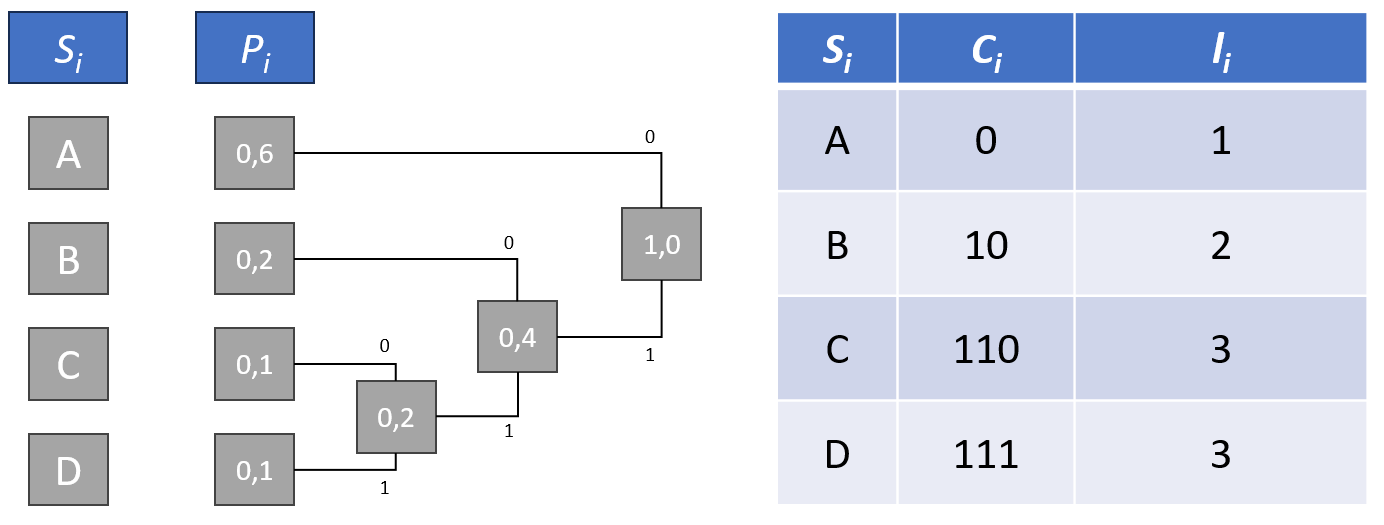
\includegraphics[scale=0.4]{Bilder/Huffmancode_beispiel.png}
  \caption[Huffman Code Beispiel]{\textbf{Erstellen eines Huffman Codes} Die Abbildung zeigt die Konstruktion eines Binärbaums und der daraus resultierenden Codewörter für die Symbole}
  \label{fig:huffman_example}
\end{figure}

\subsubsection{Resultate einer Huffman-Kodierung}
\label{subsec:huffman_res}
Aus diesem Beispiel kann der Nutzen der Huffman-Kodierung anhand von Werten ausgedrückt werden. \newline
Um die mittlere Codewortlänge einer Huffman-Kodierung zu berechnen, wird die Formel
\begin{equation*}
\bar{l} = \sum_{i=1}^{n} p_i \cdot l_i
\end{equation*}
benötigt \newline

Aus dem Beispiel ergibt sich eine mittlere Codewortlänge von 1,6 \textit{Bits/Symbol} bei einer Huffman-Kodierung.
Im Vergleich zu einem FLC werden also 0,4 \textit{Bits/Symbol} gespart. 
Die Formel für das Kompressionsverhältnis lautet:
\begin{equation*}
C_r = \frac{\text{Eingabegröße}}{\text{Ausgabegröße}}
\end{equation*}

Da sich bei einer Huffman-Kodierung lediglich die Codewortlängen ändern, kann der FLC als Eingabe-, und der Huffman Code als Ausgabegröße in der Formel verwendet werden.
So ergibt sich ein Kompressionsverhältnis von:
\begin{equation*}
C_r = \frac{\lceil \log_2(N) \rceil}{\sum_{i=1}^{n} p_i \cdot l_i}
\end{equation*}
% TODO: Problem mit Zeilenumbruch deshalb gerade zwei equations
\begin{equation*}
C_r = \frac{2,0 \ \text{Bits/Symbol}}{1,6 \ \text{Bits/Symbol}} = 1,25
\end{equation*}

Die Effektivität der Huffman-Kodierung hängt stark von der Verteilung der Symbole in der Datenquelle ab. 
Wenn der konstruierte Binärbaum stark balanciert ist, bedeutet dies, dass die Codewörter für die einzelnen Symbole ähnliche Längen haben. 
In solchen Fällen ist die Huffman-Kodierung weniger effektiv, da sie weniger Redundanz in den Daten ausnutzen kann.

Redundanz beschreibt den unnötigen Aufwand zu Repräsentation einer Information.
Wenn man eine Quelle, wie beispielsweise ein Alphabet betrachtet, spricht man von der Redundanz einer Quelle oder \textit{Quellredundanz}.
Die Quellredundanz ist abhängig von dem Entscheidungsgehalt $\mathit{H_0}$ des Alphabets und der Quellentropie $\mathit{H(X)}$.
\begin{equation*}
\Delta R_0 = H_0 - H(X)
\end{equation*}
\begin{equation*}
H_0 = \sum_{i=1}^{n} p_i * \log_2{p_i} , \quad p_i = \frac{1}{n} \ \forall i
\end{equation*}
\begin{equation*}
H_0 = \sum_{i=1}^{n} p_i * \log_2{p_i} , \quad p_i = \frac{1}{n} \ \forall i
\end{equation*}

Die Aufgabe der Huffman-Kodierung ist die Minimierung der \textit{Codierungsredundanz}.


Im Gegensatz dazu profitiert die Huffman-Kodierung enorm von einer ungleichen Verteilung der Symbole, bei der bestimmte Symbole deutlich häufiger auftreten als andere. 
Dadurch können kürzere Codewörter für häufige Symbole und längere Codewörter für seltene Symbole verwendet werden, was zu einer besseren Kompression führt.

Allerdings ist die Huffman-Kodierung anfällig für Veränderungen in der statistischen Verteilung der Symbole. 
Wenn sich die Auftrittswahrscheinlichkeiten im Laufe der Anwendung ändern oder wenn sie falsch berechnet wurden, kann dies zu einer Verschlechterung der Kompression führen. 
Im Extremfall kann es vorkommen, dass das Symbol mit der höchsten Auftrittswahrscheinlichkeit das längste Codewort erhält, was die Effizienz der Codierung erheblich beeinträchtigt. 
Daher ist es wichtig, dass die Statistik der Symbole regelmäßig überprüft und aktualisiert wird.
Um das zu bewerkstelligen kann eine adaptive Huffman-Kodierung verwendet werden. 
Anstelle einer festen Symbolstatistik wird bei der adaptiven Huffman-Kodierung die Statistik nach dem Kodieren eines Symbols überprüft und aktualisiert. 
Adaptive Algorithmen liefern zu Beginn einer Kodierung noch keine guten Ergebnisse, da die Symbolstatistik bei wenigen Symbolen nicht Aussagekräftig ist \cite{Jeon1998}. 

\subsection{GZIP}
\label{subsec:gzip}
Brotli-G misst sich mit anderen Kompressionsstandards wie GZip und Deflate.
Der Deflate Algorithmus beschreibt eine Kombination aus dem LZ77 Algorithmus und der Huffman-Kodierung
[Wahrscheinlich kein eigenes Kapitel. Lieber Deflate Algorithmus in anderen Kapiteln erwähnen]

\subsection{Brotli-G Compute Shader}
\label{subsec:brotlig_compute}
Das komprimierte Dreiecksnetz soll mittels Brotli-G's GPU Dekodierer dekodiert werden.
Da Brotli-G mit der Grafik-API DirectX12 arbeitet, wird eine GPU benötigt die das Shader Model 6 unterstützt.
Für die Verwendung des GPU Dekodierers wird also eine NVidia Grafikkarte mit der Turing-Architektur benötigt \cite{Burgess2020}.
Diese erkennt man am RTX Präfix vor der Modellnummer.
Bei AMD Grafikkarten muss mindestens die RDNA-2 Architektur verbaut sein.
Mit Grafikkarten aus der AMD RX6000er Reihe für RDNA-2, und der RX7000er Reihe für RDNA-3 kann der GPU Dekodierer verwendet werden.
Brotli-G definiert ihren GPU Dekodierer in der Shader-Sprache \textit{high-level shader language (HLSL)} und ist als Compute Shader definiert (Kap.~\ref{subsec:compute_shader}). \newline

Da es sich bei Brotli-G um eine Modifikation des Brotli Formats handelt, wurde der Bitstrom des Kodierers angepasst.


\subsection{CPU Ebene}
\label{subsec:brotlig_cpu}
Queries Buffers etc
